\documentclass[12pt, a4paper, titlepage]{jsarticle}
\usepackage[dvipdfm]{graphicx}
\usepackage{ascmac}
\begin{document}
\begin{titlepage}
\title{J3課題}
\author{1511179  前田 諒磨}
\maketitle
\end{titlepage}
\section{課題概要}
今回のドローエディターでは3x3の○×ゲームを作ろうとしました。つまりプレイヤーごとに図形の形と色を選び交互にその図形をマスに埋めていこうとしました。縦斜め横で3つ連続同じ記号にしたほうが勝ちというゲームですが、結果的には不完全になりました。実装できたことを次に上げます。
\begin{itemize}
\item 図形を楕円と長方形から選ぶ。
\item 色を3種類から選ぶ。
\item 3x3のマスを持つ。
\item マスごとに独立した図形を描ける。
\item 同じマスに図形を書こうとした際、前の図形は消える。
\end{itemize}
この中で今回の目標としたものに特に必要で、サンプルプログラムを改良したのは、マスごとに独立の図形を書けることである。
\section{設計方針}
描写したい図形において、まずはクラスFigureで図形の基本的な情報を定義して、それを継承したクラスRectangleFigureとOvalangleFigureで図形の形をそれぞれ、長方形と楕円として決めた。図形の情報はDrawModelクラスで管理した。それをViewPanelで監視した。また実際にマウスが押されたりなどした時に動くActionListenerはDrawController内に書き、ViewPanelとセットで動かした。また9つのマスそれぞれに異なる処理をさせることになったので、前述のセットを9つ用意するのにmainのあるDrawFrameには冗長になってしまうので、書かずそれ用のgameboadに書いた。また同様の理由から、色や図形を選択するcomboboxもgameboad内に書いた。
\section{プログラムの説明}
\subsection{Figureクラス}
Figureクラスのフィールド\\
int x,y,w,h はそれぞれ図形の始点の(x,y)、図形の横幅、図形の高さ。\\
Color c 図形の色

Figureクラスのメソッド\\
setSize(int w,int h) 図形の高さと横幅を設定す。\\
setLocation(int x,int y) 始点を設定します。\\
reshape(int x1,int y1,int x2,int y2) ドラッグしている情報から始点と、高さ横幅を認識する。

\subsection{RectangleFigureクラス}
RectangleFigureはFigureクラスを継承しているので、フィールドはFigureのを使っている。

RectangleFigureクラスのメソッド\\
draw(Graphics g) 色を指定した長方形を描く。
\subsection{OvalangleFigureクラス}
OvalangleFigureはRectangleFigure同様にFigureクラスを継承しており、フィールドはFigureと同じ。

OvalangleFigureクラスのメソッド\\
draw(Graphics g) 色を指定した楕円を描く。
\subsection{DrawModelクラス}
DrawModelのフィールド\\
Figure drawingFigure  描かれる図形を記憶する。(今回サンプルコードと違い一つのモデルに一つだけ記憶すれば良いのでArrayListは使っていない)\\
Color currentColor  描かれる図形の色を格納する。\\

DrawModelのメソッド\\
setColor (Color c) 図形の色を変更する。\\
createRectFigure(int x, int y) RectangleFigureを利用して長方形を描き記憶する。\\
createOvalFigure(int x, int y) OvalangleFigureを利用して楕円を描き記憶する。\\
reshapeFigure(int x1,int y1,int x2,int y2) ある図形のFigureのreshapeメソッドを利用する。\\
\subsection{ViewPanelクラス}
ViewPanelのフィールド\\
DrawModel model DrawModel参照\\

ViewPanelのメソッド\\
paintComponent(Graphics g) 図形の表示\\
update(Observable o, Object arg) modelに変更があればupdate

\subsection{Drawcontrollerクラス}
DrawControllerのフィールド\\
DrawModel model DrawModel参照\\
int dragStartX, dragStartY ドラッグ開始時の座標XとY\\
int i 図形選択のための整数。この値を外から変えて図形を変更する。\\

DrawControllerのメソッド\\
setnum(int n) 図形選択のためのiを変更して図形を確定。\\
mousePressed(MouseEvent e) マウスクリック時の動作。\\
mouseDragged(MouseEvent e) マウスドラッグ時の動作。\\

このクラスのマウスのイベント内ではiを用いてどの図形を呼ぶのかを制御している。
\subsection{gameboadクラス}
gameboadのフィールド(数字 ~ 数字となっているのは数が多いので省略してあり、それぞれ同じ意味で使用されている。)\\
JPanel p 3x3のマスを定義するためのJPanel\\
DrawModel model1~9 マスごとに異なるmodelを定義するためのmodel\\
ViewPanel view1~9 上と同様\\
DrawController cont1~9 上と同様\\
String[] cmlist1 = { "red", "blue", "yellow" }, cmlist2 = { "四角", "円" } combobox内の選択肢のリスト\\
JToolBar tb ツールバー\\
JComboBox cm1, cm2 図形と色を選択するためのcombobox\\

gameboadのメソッド\\
actionPerformed(ActionEvent e) Jcomboboxが変更された時に実行する。各変更を9つ全てに適応させている。\\

このクラスはサンプルコードにはなく、9つのマスを独立させるために、作成した。DrawFrame内でも書けたが、同じことの繰り返しで長くなっているので、見やすくするために分けた。また、comboboxと同じクラスにしておくと、図形の選択を反映させるのが楽であると思い、同包した。
\subsection{DrawFrameクラス}
DrawFrameのフィールド\\
gameboad gb gameboad参照

このクラスはGUIの実際に見える部分の配置とメイン関数を持っている。コンストラクタで配置をしている。ここでgbの中身を配置する上で、Panelとツールバー両方を忘れないようにgb.でaddして配置している。\\
メイン関数は自分自身を実行しているだけである。

\subsection{プログラム全体}
mvcモデルとしてDrawModel, ViewPanel, DrawControllerを作成しそれぞれを作用させて、それらを9セット宣言して配置することで、各マスを独立させ、更に中に描く図形もいじれるようにしたことで、3x3のゲームを作れる準備ができている。


\section{実行例}
まずはDrawEditor上部のボックスから適当に色や図形を変更して描いたものです。(図1)

\begin{figure}[htbp]
 \begin{center}
 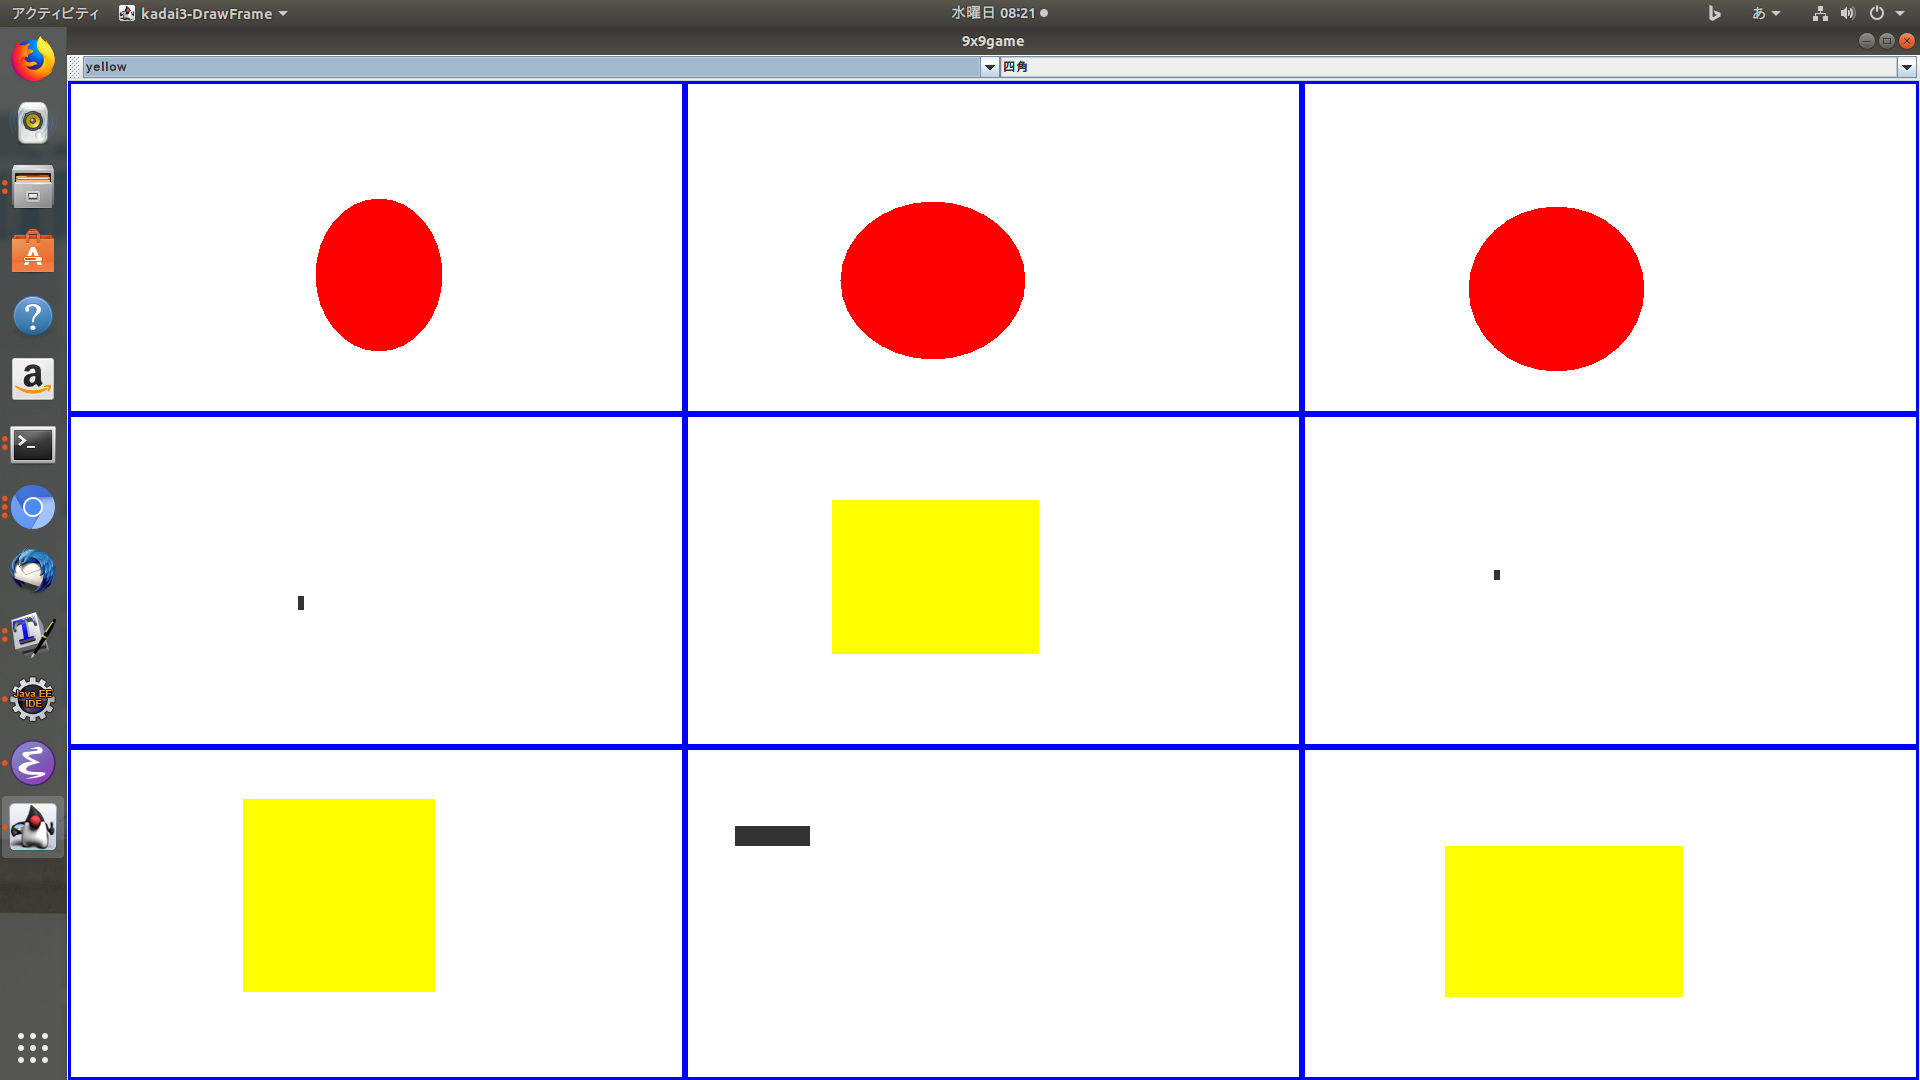
\includegraphics[width=10cm,clip]{kekka1.png}
 \end{center}
 \caption{実行例1}
\end{figure}

次に色をblueにして図形を四角にして中心の上のマスに四角を描いてみる。(図2)

\begin{figure}[htbp]
 \begin{center}
 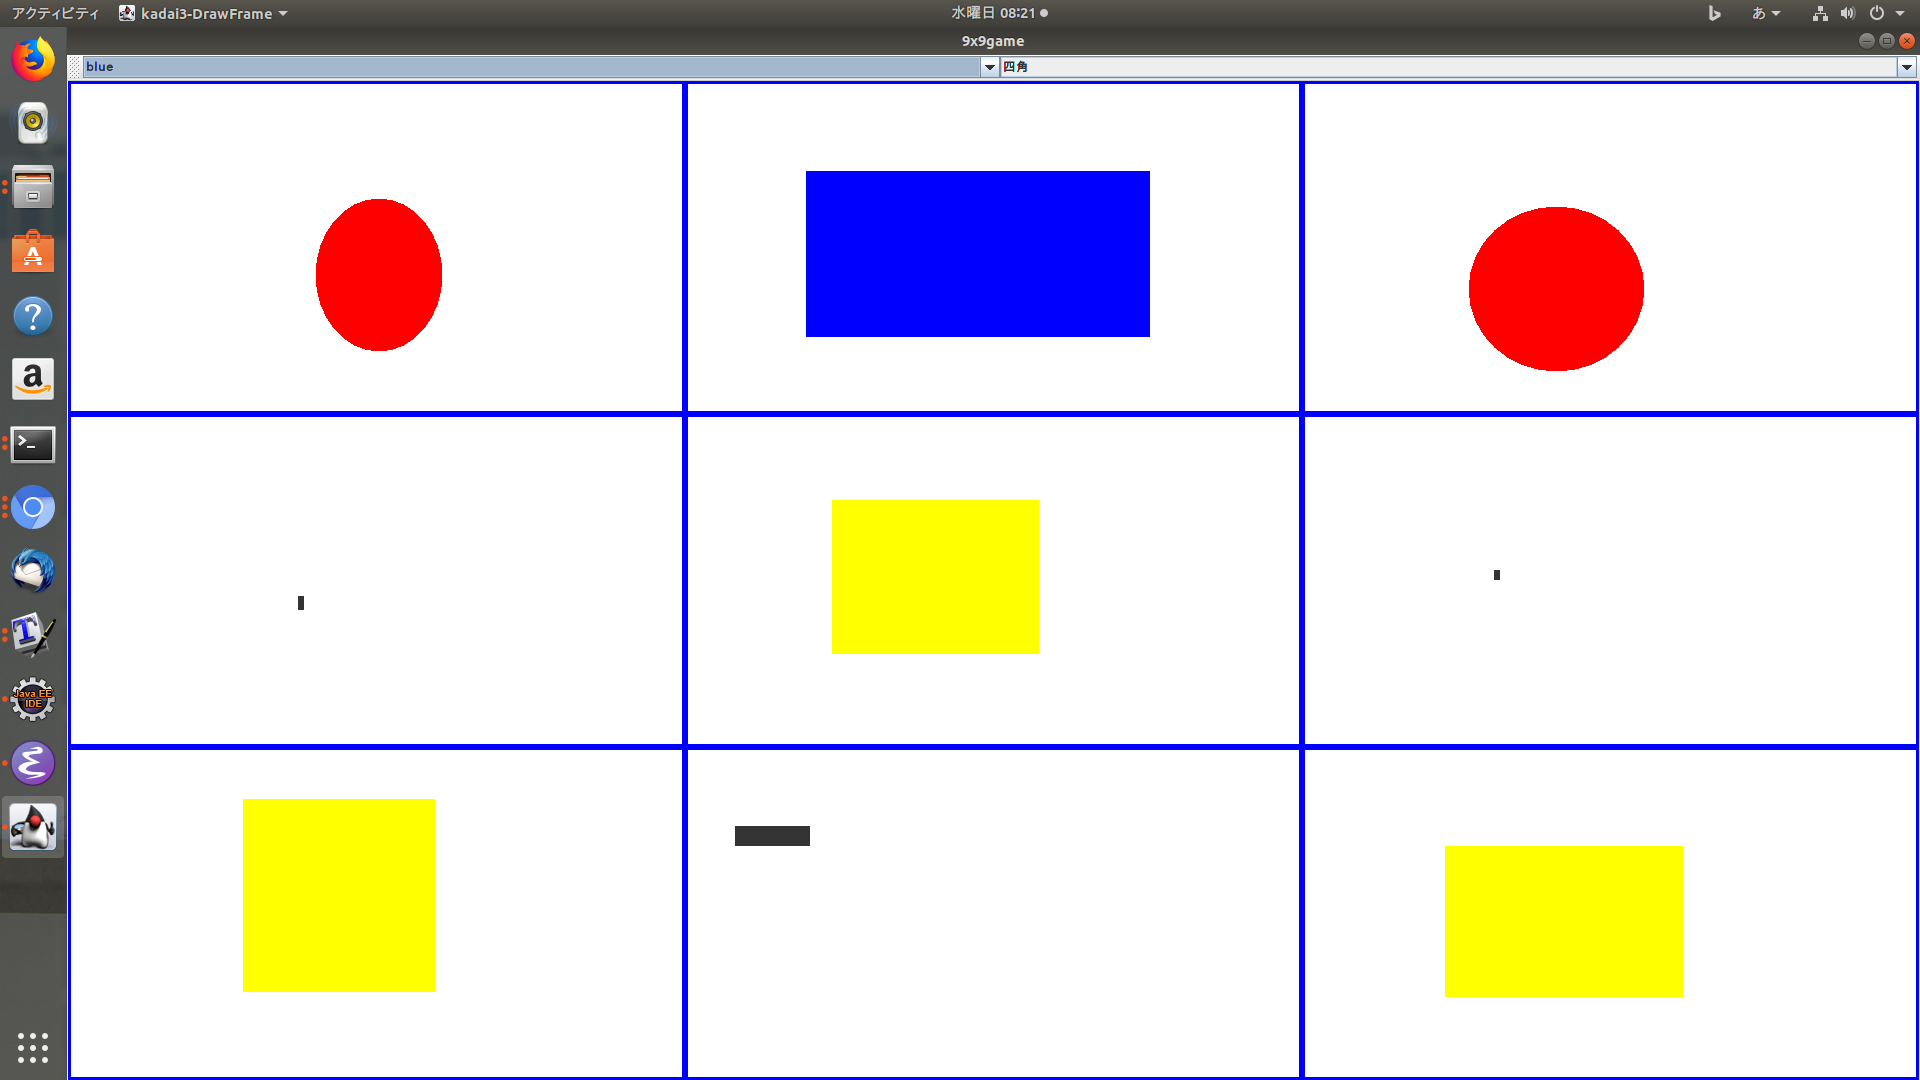
\includegraphics[width=10cm,clip]{kekka2.png}
 \end{center}
 \caption{実行例2}
\end{figure}

これはマス一つに一つの図形なので、前の赤い楕円が消えている。
\section{考察}
今回の課題で目標としたものには全然届かなかった。独立で動きはしていたが、仮に最初に述べたゲームを行うとすると、毎回図形か色、または両方を変更してかつ一度描いたマスには、上から描かないという、ユーザー側の努力が必要になってしまった。

本来目指していたインターフェースはツールバーにはplayer1 とplayer2の図形と色を定義する場所を設ける。つまりツールバーをGridLayout(1,6)に区切って2種類の図形を決める場所をつけて、一回クリックするごとに図形が代わりかつ1度図形を追加したマスには追加できないようにしようとしたが、実行するのに、クリックごとに図形が変える方法が思いつかなかった。

また、全部をリセットするボタンもつけれたら更に有用であった。これには時間がなかったが、おそらくmodelの部分で初期化するメソッドを持たせて、初期化の際、前9つのmodelでそれを実行すればできたと考えられる。
\section{感想}
今回の課題はこの大学では珍しいGUIの勉強で楽しめたが。思っていた以上に実装しようとしたことが、その方法が思いつかず不完全に終わってしまった。もう少し余裕を持って調べながらすすめるべきであったと思う。
また突然今までとは違う言語だったが、プログラム自体に耐性が少しはできたのか、学びやすかった気がした。
\section{操作法}
実行例の時に使った画像であるがこれを使って説明する。
\begin{figure}[htbp]
 \begin{center}
 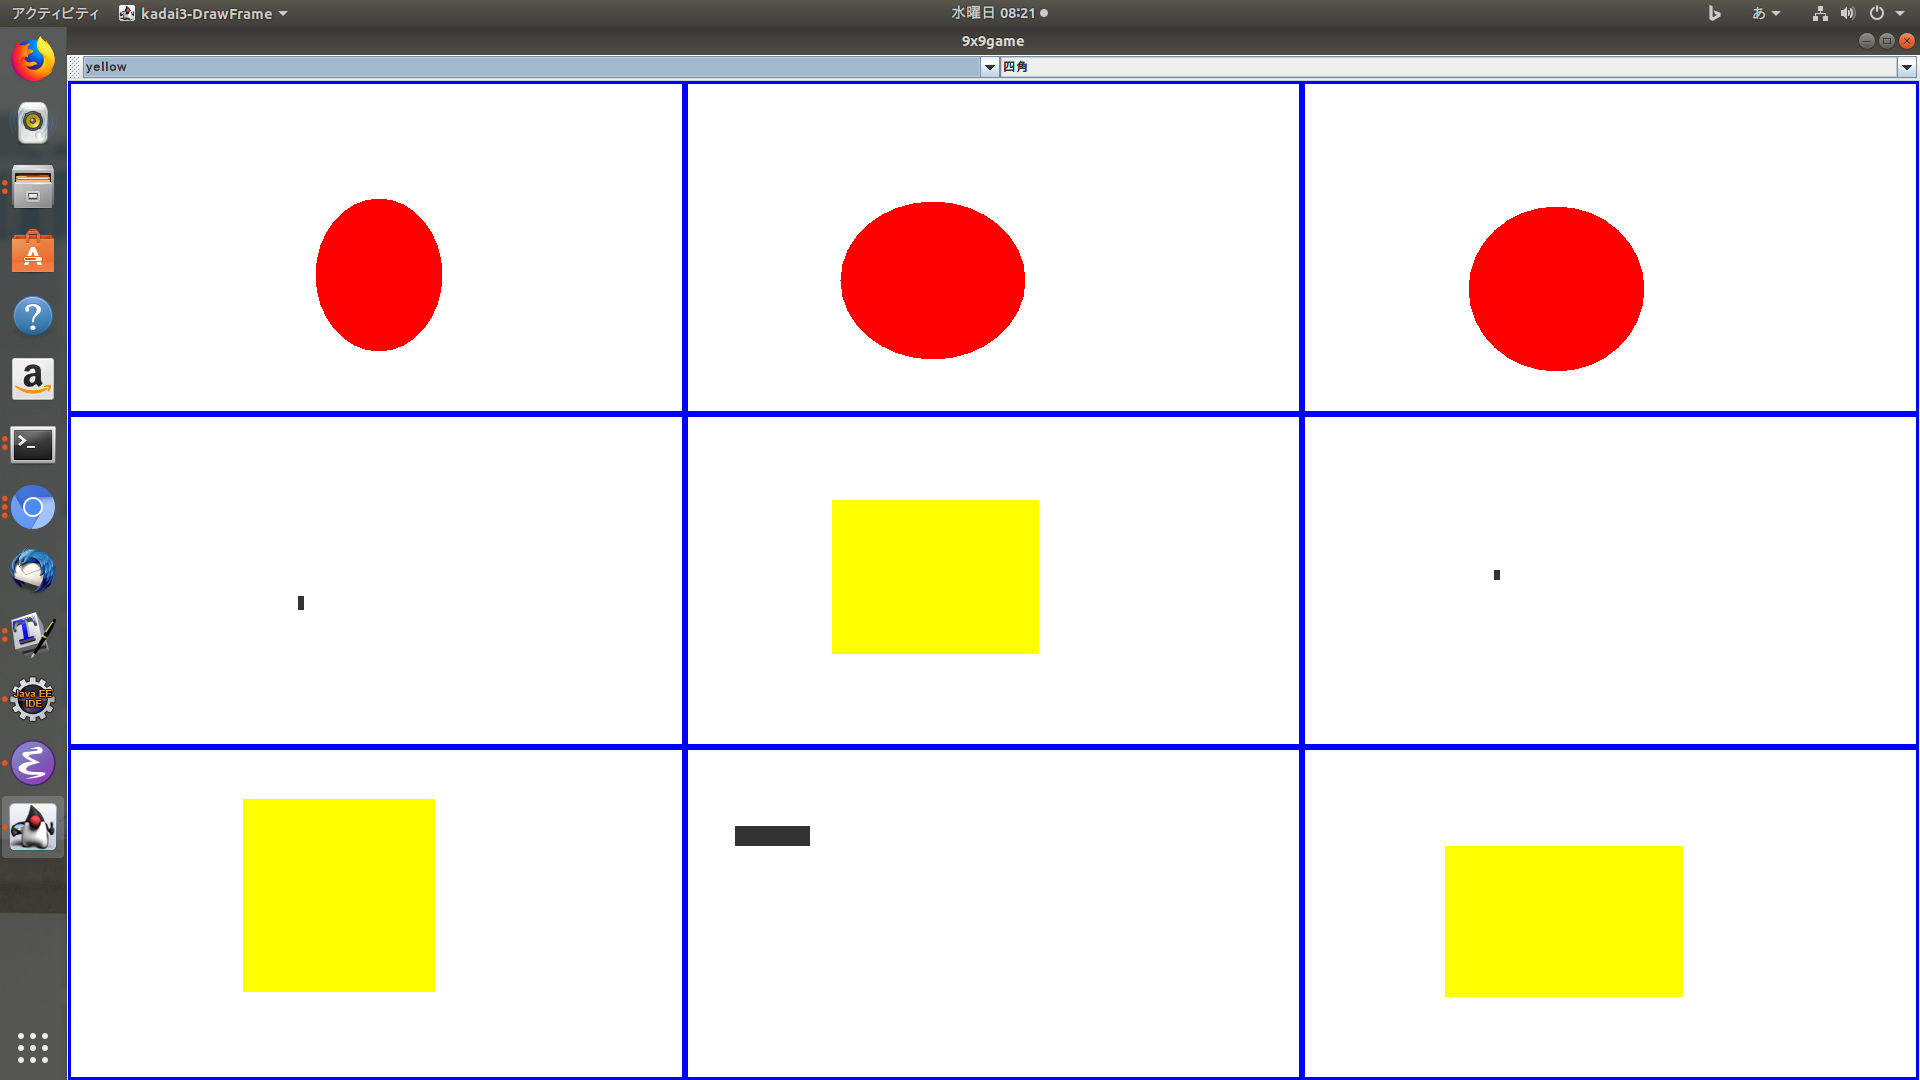
\includegraphics[width=10cm,clip]{kekka1.png}
 \end{center}
 \caption{実行例1}
\end{figure}

\subsection{図形の変更}
上部のツールバーに2つのボックスがあり、画像では左からyellow,四角となっているが、左がその後描く図形の色を、右が形を決めることができる。
\subsection{図形の描写}
それぞれ9つのマスは独立なので、マス内でスタートしたい場所から好きな大きさにドラッグして図形を表示する。
\subsection{図形の上書き}
すでに図形の存在するマスに図形の描写の時と同じようにしたら、前の図形は消え、新しい図形が描ける。このとき前のと新しい図形は色も形も違っていても大丈夫である。

\section{ソースコード}
eclipseを利用しているためclassごとに区切って載せておく。
\begin{screen}
\begin{verbatim}
package kadai3;

import javax.swing.*;
import java.awt.*;
import java.awt.event.*;

class Figure {
	protected int x,y,width,height;
	protected Color color;
	public Figure(int x,int y,int w,int h,Color c) {
		  this.x = x; this.y = y;  // this.x, this.y はインスタンス変数を指します.
		  width = w; height = h;   // ローカル変数で同名の変数がある場合は,this
		  color = c;               // を付けると,インスタンス変数を指すことになります.
		}
	public void setSize(int w,int h) {
		  width = w; height = h;
		}
	public void setLocation(int x,int y) {
		  this.x = x; this.y = y;
		}
	public void reshape(int x1,int y1,int x2,int y2) {
		  int newx = Math.min(x1,x2);
		  int newy = Math.min(y1,y2);
		  int neww = Math.abs(x1-x2);
		  int newh = Math.abs(y1-y2);
		  setLocation(newx,newy);
		  setSize(neww,newh);
		}
	public void draw(Graphics g) {}
}

\end{verbatim}
\end{screen}
\begin{screen}
\begin{verbatim}
package kadai3;
import javax.swing.*;
import java.awt.*;
import java.awt.event.*;

public class RectangleFigure extends Figure{
	public RectangleFigure(int x,int y,int w,int h,Color c) {
	    super(x,y,w,h,c);
	    // 引数付きのコンストラクタは継承されないので,コンストラクタを定義.
	    // superで親のコンストラクタを呼び出すだけ.
	  }
	  public void draw(Graphics g) {
	    g.setColor(color);
	    g.fillRect(x,y,width,height);
	  }

	  
	  
}

\end{verbatim}
\end{screen}
\begin{screen}
\begin{verbatim}
package kadai3;
import javax.swing.*;
import java.awt.*;
import java.awt.event.*;

public class OvalangleFigure extends Figure{
	public OvalangleFigure(int x,int y,int w,int h,Color c) {
	    super(x,y,w,h,c);
	    // 引数付きのコンストラクタは継承されないので,コンストラクタを定義.
	    // superで親のコンストラクタを呼び出すだけ.
	  }
	  public void draw(Graphics g) {
	    g.setColor(color);
	    g.fillOval(x,y,width,height);
	  }
}

\end{verbatim}
\end{screen}
\begin{screen}
\begin{verbatim}
package kadai3;

import java.util.*;
import javax.swing.*;
import java.awt.*;
import java.awt.event.*;

public class DrawModel extends Observable{

	  protected Figure drawingFigure;
	  protected Color currentColor;
	  public void DrawModel() { 
		  currentColor = Color.red;
		  Figure f = null;
		 
	  }
	  
	  public void setColor (Color c) {
		  currentColor = c; 
	  }
	  
	
	public void createRectFigure(int x, int y) {
			Figure f = new RectangleFigure(x, y, 0, 0, currentColor);
			drawingFigure = f;
			setChanged();
			notifyObservers();
		
	}
\end{verbatim}
\end{screen}
\begin{screen}
\begin{verbatim}
	public void createOvalFigure(int x, int y) {
			Figure f = new OvalangleFigure(x, y, 0, 0, currentColor);
			drawingFigure = f;
			setChanged();
			notifyObservers();
	}
	  public void reshapeFigure(int x1,int y1,int x2,int y2) {
	      drawingFigure.reshape(x1,y1,x2,y2);
	      setChanged();
	      notifyObservers();
	  }
	
	
}

\end{verbatim}
\end{screen}
\begin{screen}
\begin{verbatim}
package kadai3;

import java.util.*;
import javax.swing.*;
import java.awt.*;
import java.awt.event.*;

public class ViewPanel extends JPanel implements Observer {

	protected DrawModel model;

	public ViewPanel(DrawModel m, DrawController c) {
		this.setBackground(Color.white);
		this.addMouseListener(c);
		this.addMouseMotionListener(c);
		model = m;
		model.addObserver(this);
		
	}

	public void paintComponent(Graphics g) {
		super.paintComponent(g);
		Figure f = model.drawingFigure;
		f.draw(g);
	}

	public void update(Observable o, Object arg) {
		repaint();
	}

}

\end{verbatim}
\end{screen}
\begin{screen}
\begin{verbatim}
package kadai3;

import java.util.*;
import javax.swing.*;
import java.awt.*;
import java.awt.event.*;

public class DrawController implements MouseListener, MouseMotionListener {
	protected DrawModel model;
	protected int dragStartX, dragStartY;
	int i;

	public DrawController(DrawModel a) {
		model = a;
		i = 0;
	}

	public void setnum(int n) {
		i = n;
	}
	
	public void mouseClicked(MouseEvent e) {
	}

	public void mousePressed(MouseEvent e) {
		dragStartX = e.getX();
		dragStartY = e.getY();
		if(i == 0)
		model.createRectFigure(dragStartX, dragStartY);
		if(i == 1)
			model.createOvalFigure(dragStartX, dragStartY);
	}
\end{verbatim}
\end{screen}
\begin{screen}
\begin{verbatim}
	public void mouseDragged(MouseEvent e) {
		model.reshapeFigure(dragStartX, dragStartY, e.getX(), e.getY());
	}

	public void mouseReleased(MouseEvent e) {
	}

	public void mouseEntered(MouseEvent e) {
	}

	public void mouseExited(MouseEvent e) {
	}

	public void mouseMoved(MouseEvent e) {
	}
}

\end{verbatim}
\end{screen}
\begin{screen}
\begin{verbatim}
package kadai3;

import javax.swing.*;
import java.awt.*;
import java.awt.event.*;
import javax.swing.border.LineBorder;

public class gameboad extends JFrame implements ActionListener {
	JPanel p;
	DrawModel model1, model2, model3, model4, model5, model6, model7, model8, model9;
	ViewPanel view1, view2, view3, view4, view5, view6, view7, view8, view9;
	DrawController cont1, cont2, cont3, cont4, cont5, cont6, cont7, cont8, cont9;
	String[] cmlist1 = { "red", "blue", "yellow" }, cmlist2 = { "四角", "円" };
	JToolBar tb;
	JComboBox cm1, cm2;

	public gameboad() {
		model1 = new DrawModel();
		model2 = new DrawModel();
		model3 = new DrawModel();
		model4 = new DrawModel();
		model5 = new DrawModel();
		model6 = new DrawModel();
		model7 = new DrawModel();
		model8 = new DrawModel();
		model9 = new DrawModel();
		cont1 = new DrawController(model1);
		cont2 = new DrawController(model2);
		cont3 = new DrawController(model3);
		cont4 = new DrawController(model4);
		cont5 = new DrawController(model5);
\end{verbatim}
\end{screen}
\begin{screen}
\begin{verbatim}
		cont6 = new DrawController(model6);
		cont7 = new DrawController(model7);
		cont8 = new DrawController(model8);
		cont9 = new DrawController(model9);
		view1 = new ViewPanel(model1, cont1);
		view2 = new ViewPanel(model2, cont2);
		view3 = new ViewPanel(model3, cont3);
		view4 = new ViewPanel(model4, cont4);
		view5 = new ViewPanel(model5, cont5);
		view6 = new ViewPanel(model6, cont6);
		view7 = new ViewPanel(model7, cont7);
		view8 = new ViewPanel(model8, cont8);
		view9 = new ViewPanel(model9, cont9);
		view1.setBorder(new LineBorder(Color.blue, 3));
		view2.setBorder(new LineBorder(Color.blue, 3));
		view3.setBorder(new LineBorder(Color.blue, 3));
		view4.setBorder(new LineBorder(Color.blue, 3));
		view5.setBorder(new LineBorder(Color.blue, 3));
		view6.setBorder(new LineBorder(Color.blue, 3));
		view7.setBorder(new LineBorder(Color.blue, 3));
		view8.setBorder(new LineBorder(Color.blue, 3));
		view9.setBorder(new LineBorder(Color.blue, 3));
		p = new JPanel();
		p.setLayout(new GridLayout(3, 3));
		p.add(view1);
		p.add(view2);
		p.add(view3);
		p.add(view4);
		p.add(view5);
		p.add(view6);
		p.add(view7);
		p.add(view8);
		p.add(view9);
\end{verbatim}
\end{screen}
\begin{screen}
\begin{verbatim}
		tb = new JToolBar();
		tb.setLayout(new GridLayout(1, 2));
		cm1 = new JComboBox(cmlist1);
		cm2 = new JComboBox(cmlist2);
		tb.add(cm1);
		tb.add(cm2);
		cm1.addActionListener(this);
		cm2.addActionListener(this);
	}

	public void actionPerformed(ActionEvent e) {
		if (cm1.getSelectedIndex() == 0) {
			model1.setColor(Color.red);
			model2.setColor(Color.red);
			model3.setColor(Color.red);
			model4.setColor(Color.red);
			model5.setColor(Color.red);
			model6.setColor(Color.red);
			model7.setColor(Color.red);
			model8.setColor(Color.red);
			model9.setColor(Color.red);
		} 
		else if (cm1.getSelectedIndex() == 1) {
			model1.setColor(Color.blue);
			model2.setColor(Color.blue);
			model3.setColor(Color.blue);
			model4.setColor(Color.blue);
			model5.setColor(Color.blue);
			model6.setColor(Color.blue);
			model7.setColor(Color.blue);
			model8.setColor(Color.blue);
			model9.setColor(Color.blue);
		} 
\end{verbatim}
\end{screen}
\begin{screen}
\begin{verbatim}
		else if (cm1.getSelectedIndex() == 2) {
			model1.setColor(Color.yellow);
			model2.setColor(Color.yellow);
			model3.setColor(Color.yellow);
			model4.setColor(Color.yellow);
			model5.setColor(Color.yellow);
			model6.setColor(Color.yellow);
			model7.setColor(Color.yellow);
			model8.setColor(Color.yellow);
			model9.setColor(Color.yellow);
		} 
		if (cm2.getSelectedIndex() == 0) {
			cont1.setnum(0);
			cont2.setnum(0);
			cont3.setnum(0);
			cont4.setnum(0);
			cont5.setnum(0);
			cont6.setnum(0);
			cont7.setnum(0);
			cont8.setnum(0);
			cont9.setnum(0);
		}
		else if(cm2.getSelectedIndex() == 1) {
			cont1.setnum(1);
			cont2.setnum(1);
			cont3.setnum(1);
			cont4.setnum(1);
			cont5.setnum(1);
			cont6.setnum(1);
			cont7.setnum(1);
			cont8.setnum(1);
			cont9.setnum(1);
		}
	}

}
\end{verbatim}
\end{screen}
\begin{screen}
\begin{verbatim}
package kadai3;

import java.util.*;
import javax.swing.*;
import java.awt.*;
import java.awt.event.*;
import javax.swing.border.*;

public class DrawFrame extends JFrame {
	
	gameboad gb;
	
	public DrawFrame() {
		gb = new gameboad();
		
		
		
		this.setBackground(Color.black);
		this.setTitle("9x9game");
		this.setSize(1500, 1000);
		
		
		this.add(gb.p,BorderLayout.CENTER);
		this.add(gb.tb,BorderLayout.NORTH);
		this.setDefaultCloseOperation(JFrame.EXIT_ON_CLOSE);
		this.setVisible(true);
	}

	public static void main(String argv[]) {
		new DrawFrame();
	}
}

\end{verbatim}
\end{screen}
\end{document}